\section{Dise\~no de bajo nivel}
\label{lld}  
  \subsection{Clases concretas}
  En esta secci\'on se presentan las clases concretas que implementan las
interfaces presentadas en la secci\'on~\ref{hld}. Para mayor claridad, se
dividieron los diagramas UML por paquetes.

  \subsubsection{Combinatory}
  En la Figura~\ref{uml:lld-combinatory} se puede ver el diagrama de clases
para el paquete ``Combinatory''.
    \begin{figure}
      \centering
      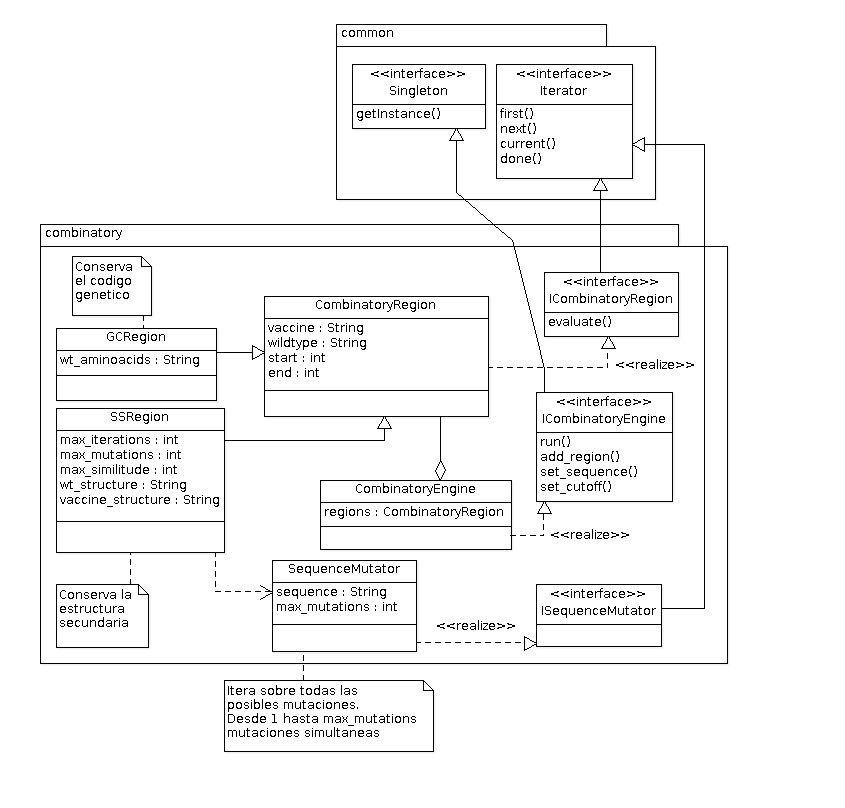
\includegraphics[scale=0.5]{lld-combinatory.png}  
      \caption{UML - Combinatory}
      \label{uml:lld-combinatory}
    \end{figure}

  \subsubsection{Validator}
  En la Figura~\ref{uml:lld-validator} se puede ver el diagrama de clases
para el paquete ``Validator''.
    \begin{figure}
      \centering
      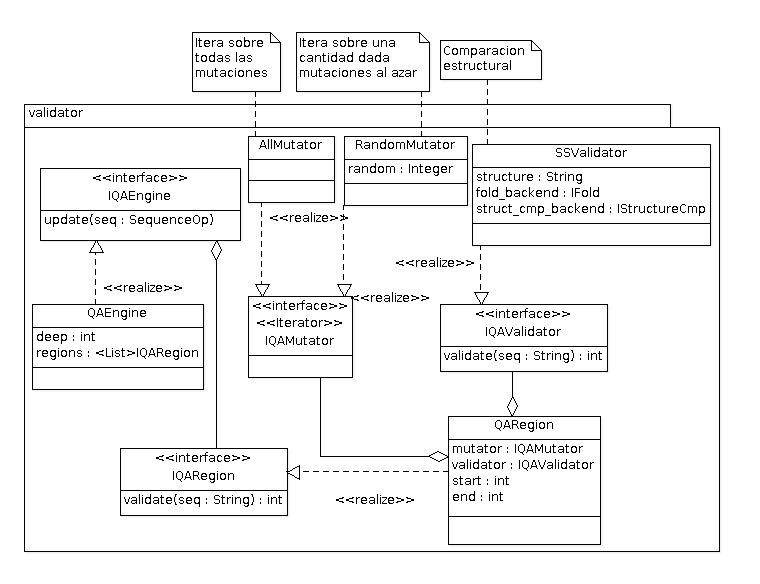
\includegraphics[scale=0.5]{lld-validator.png}  
      \caption{UML - Validator}
      \label{uml:lld-validator}
    \end{figure}